%%%%%%%%%%%%%%%%%%%%%%%%%%%%%%%%%%%%%%%%%%%%%%%%%%%%%%%%%%%%%%%%%%%%%%%%%%%%%%%%%%%%%%%%%%%%%
%%%%%%%%    This is a modified version of the ICML 2021 template     %%%%%%%%%%%%%%%%%%%%%%%%
%%%%%%%% Link: https://www.overleaf.com/latex/templates/icml2021-template/dsftnbmjgyhv %%%%%%
%%%%%%%%%%%%%%%%%%%%%%%%%%%%%%%%%%%%%%%%%%%%%%%%%%%%%%%%%%%%%%%%%%%%%%%%%%%%%%%%%%%%%%%%%%%%%

\documentclass{article}

\usepackage{microtype}
\usepackage{graphicx}
\usepackage{subfigure}
\usepackage{booktabs}
\usepackage{amsmath,amssymb}
\usepackage{array}
\usepackage{tikz}
\usetikzlibrary{positioning, calc, fit, backgrounds, shapes.geometric, arrows.meta}

\usepackage[hypertexnames=false]{hyperref}

\newcommand{\theHalgorithm}{\arabic{algorithm}}
\newcolumntype{L}[1]{>{\raggedright\arraybackslash}p{#1}}

\usepackage[accepted]{icml2021}

\begin{document}

\twocolumn[
\icmltitle{EagleVision: Lightweight Geometric Adaptation for Monocular Depth Estimation}

\begin{icmlauthorlist}
\icmlauthor{Mohammad Ali Wajid}{}
\icmlauthor{Muhammad Ammar Anees}{}
\end{icmlauthorlist}

\icmlkeywords{Machine Learning, Depth Estimation, Geometric Consistency}

\vskip 0.3in
]

\begin{abstract}
Modern monocular depth estimators are highly capable in single-view settings \cite{eigen2014depth,ranftl2022midas,yang2024depthanything,yang2024depthanythingv2}, but cross-view geometric consistency remains a practical gap in RGB-D pipelines that rely on camera motion and reprojection. We present \textbf{EagleVision}, a lightweight adaptation framework that keeps a standard pretrained Depth Anything V2 model \cite{yang2024depthanythingv2} frozen and learns only a compact residual adapter under a round-trip geometric objective. The key design is to correct, not replace, pretrained depth: the adapter predicts residual refinements, and consistency is enforced through explicit source$\rightarrow$target$\rightarrow$source warping. We train the final model for 100 epochs on the ScanNet domain \cite{dai2017scannet} and evaluate it against frozen Depth Anything V2 under aligned paired protocols, then study cross-model behavior under a multi-model evaluation setting on NYU/KITTI-style benchmarks \cite{silberman2012nyu,geiger2012kitti}. EagleVision improves core depth and geometry metrics while preserving a small trainable footprint, with remaining gaps mainly tied to sparse warping coverage and visibility holes. Project page and code: \href{https://github.com/<ORG>/<REPO>}{\texttt{[GitHub link placeholder]}}.
\end{abstract}

\section{Introduction}
Monocular depth estimation has progressed rapidly through large-scale pretraining and transformer backbones \cite{dosovitskiy2021vit,oquab2023dinov2,ranftl2021dpt,ranftl2022midas,yang2024depthanything,yang2024depthanythingv2}, with Depth Anything V2 \cite{yang2024depthanythingv2} representing a strong and widely used baseline. At the same time, many real pipelines consume depth in \emph{multi-view} contexts rather than single-image isolation. In indoor RGB-D settings, predicted depth is repeatedly used for reprojection, geometric warping, and view-to-view consistency checks. This creates a recurring gap: a model can be strong in frame-wise depth quality yet still be weak in geometric agreement across nearby camera poses.

Recent work in depth adaptation and geometry-aware training has explored full fine-tuning, self-supervised consistency objectives, and multi-term reconstruction losses \cite{godard2019monodepth2,ranftl2022midas,bhat2023zoedepth}. These approaches are effective but often expensive or unstable when compute is constrained, and they may overwrite useful pretrained priors. Our motivation is therefore practical: keep the pretrained model intact, and learn only the smallest correction needed to satisfy geometric consistency in the target domain.

EagleVision is designed around that motivation. We treat Depth Anything V2 \cite{yang2024depthanythingv2} as a standard off-the-shelf backbone, freeze it, and attach a lightweight residual head in the spirit of parameter-efficient adaptation \cite{houlsby2019adapters}. The residual head is trained under an explicit round-trip geometric objective so that corrected depth is not only accurate in target view space, but also coherent after backward reprojection to source view space. This paper focuses on the final 100-epoch ScanNet-trained model \cite{dai2017scannet} and its comparison against frozen Depth Anything V2 under controlled evaluation protocols.

\textbf{Contributions.}
\begin{itemize}
  \item A lightweight residual adaptation strategy for monocular depth that preserves a frozen standard backbone.
  \item A geometry-grounded round-trip training objective that couples forward and backward warping consistency.
  \item A complete evaluation protocol including ablation-based hyperparameter selection, ScanNet-domain quantitative comparison against frozen Depth Anything V2, and multi-model cross-dataset benchmarking.
\end{itemize}

\section{Methodology}
\subsection{Overview}
EagleVision has three functional components: (1) a frozen pretrained depth backbone, (2) a small trainable residual adapter, and (3) an explicit geometric warping module. The backbone supplies base depth, the adapter predicts a correction, and the round-trip warp loop provides cross-view geometric supervision. Figure~\ref{fig:eaglevision_block} summarizes the exact forward pass used during training and evaluation.

\begin{figure*}[t]
\centering
\resizebox{0.98\textwidth}{!}{%
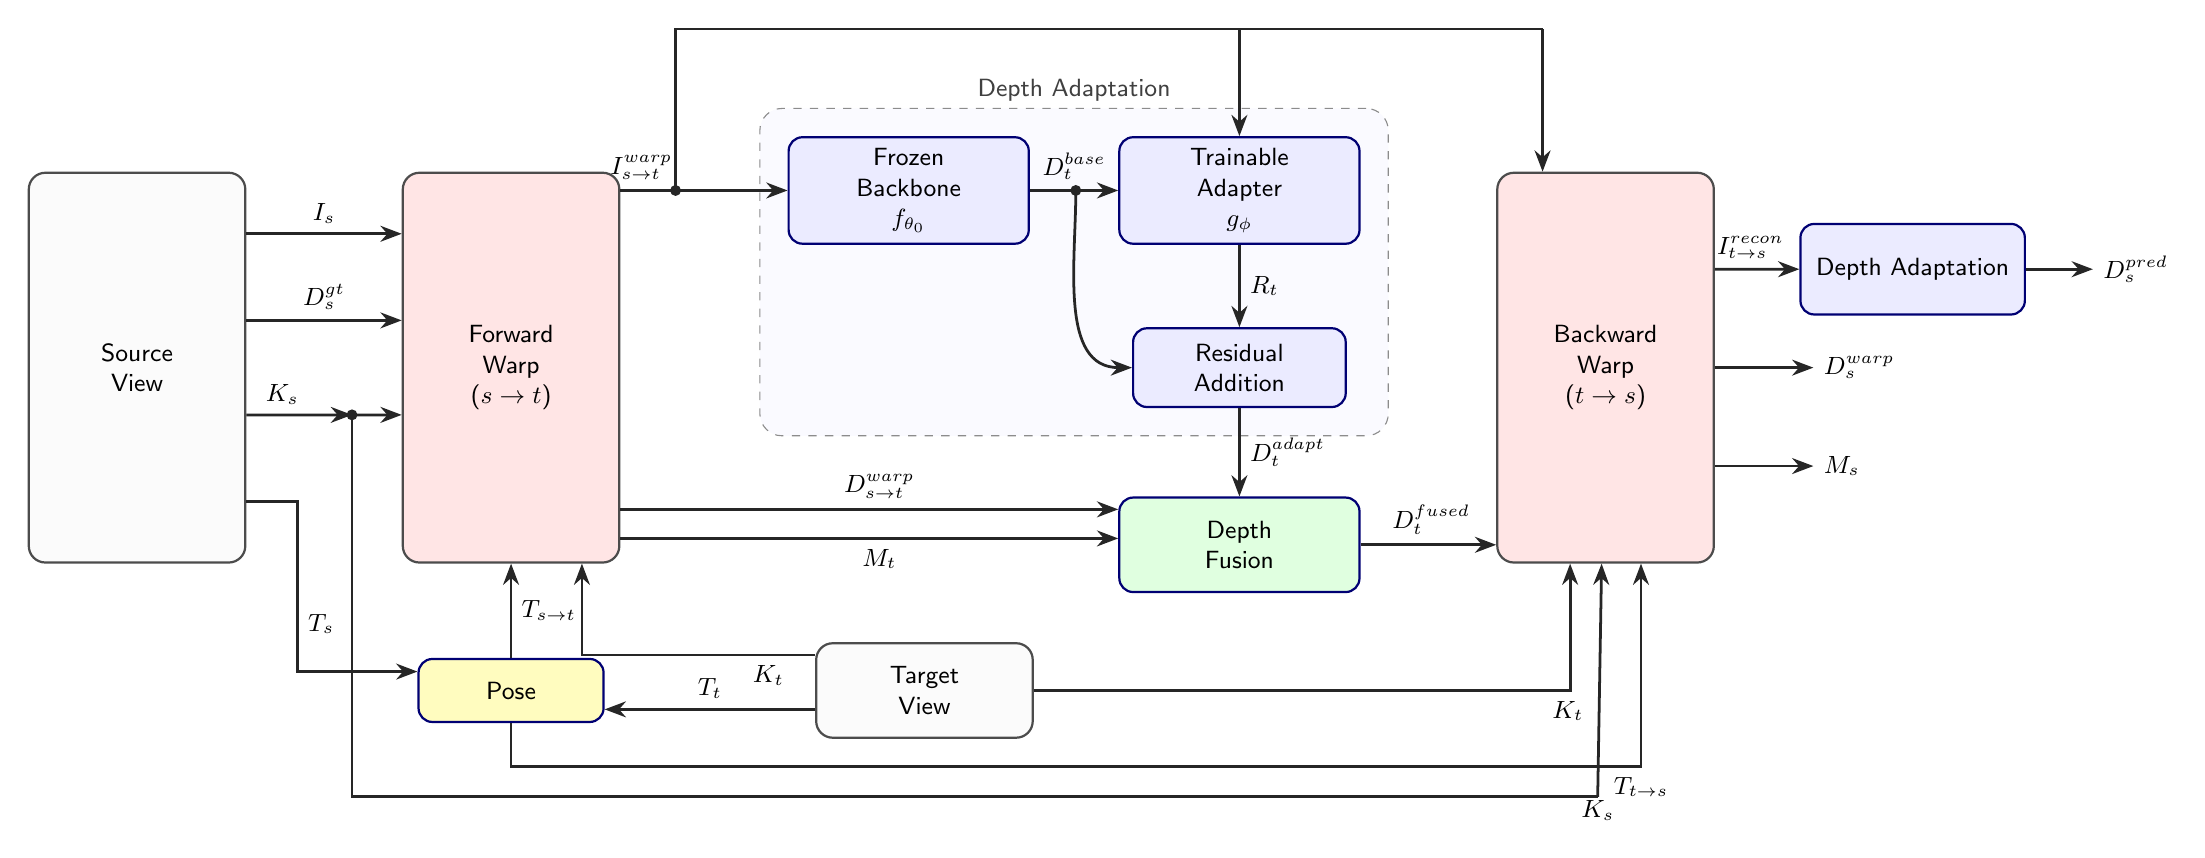
\begin{tikzpicture}[x=1cm,y=1cm]

    \tikzset{
        stage/.style={
            rectangle,
            draw=black!70,
            rounded corners=6pt,
            minimum width=2.75cm,
            minimum height=4.95cm,
            align=center,
            thick,
            inner sep=6pt,
            fill=gray!3,
            font=\sffamily\small
        },
        stage_warp/.style={
            stage,
            fill=red!10
        },
        module_pose/.style={
            module_small,
            fill=yellow!25
        },
        module_fusion/.style={
            module,
            fill=green!12
        },
        stage_small/.style={
            stage,
            minimum height=1.2cm,
            minimum width=2.75cm
        },
        module/.style={
            rectangle,
            draw=blue!45!black,
            rounded corners=5pt,
            minimum width=3.05cm,
            minimum height=1.2cm,
            align=center,
            thick,
            inner sep=4pt,
            fill=blue!8,
            font=\sffamily\small
        },
        module_small/.style={
            module,
            minimum width=2.7cm,
            minimum height=1cm
        },
        group_box/.style={
            draw=black!45,
            rounded corners=8pt,
            dashed,
            inner sep=10pt,
            fill=blue!2
        },
        arrow/.style={
            line width=1pt,
            -{Stealth[length=2.7mm]},
            draw=black!85
        },
        wire/.style={
            line width=1pt,
            draw=black!85
        },
        data/.style={
            font=\small
        },
        group_label/.style={
            font=\sffamily\small,
            inner sep=2pt,
            fill=white,
            text=black!75
        },
        junction/.style={
            circle,
            fill=black!85,
            inner sep=1.4pt
        }
    }

    \node (source) [stage] at (0,0) {Source\\View};
    \node (target) [stage_small] at (10.0,-4.1) {Target\\View};
    \node (pose) [module_pose, minimum width=2.35cm, minimum height=0.8cm] at (4.75,-4.1) {Pose};
    \node (forward) [stage_warp] at (4.75,0) {Forward\\Warp\\($s\to t$)};
    \node (backbone) [module] at (9.8,2.25) {Frozen\\Backbone\\$f_{\theta_0}$};
    \node (adapter) [module] at (14.0,2.25) {Trainable\\Adapter\\$g_{\phi}$};
    \node (residual) [module_small] at (14.0,0) {Residual\\Addition};
    \node (fusion) [module_fusion] at (14.0,-2.25) {Depth\\Fusion};
    \node (backward) [stage_warp] at (18.65,0) {Backward\\Warp\\($t\to s$)};
    \node (shared_est) [module_small, minimum width=2.85cm, minimum height=1.15cm] at (22.55,1.25) {Depth Adaptation};

    \begin{scope}[on background layer]
        \node (adapt_box) [
            group_box,
            fit=(backbone)(adapter)(residual),
            label={[group_label]above:Depth Adaptation}
        ] {};
    \end{scope}

    \coordinate (sf1) at ([yshift=1.7cm]source.east);
    \coordinate (sf2) at ([yshift=0.6cm]source.east);
    \coordinate (sf3) at ([yshift=-0.6cm]source.east);
    \coordinate (sf3_end) at (sf3 -| forward.west);
    \coordinate (ks_split) at ($(sf3)!0.68!(sf3_end)$);
    \coordinate (ks_branch_drop) at ($(ks_split)+(0,-4.85cm)$);
    \coordinate (ks_branch_run) at ([xshift=-0.1cm]backward.south |- ks_branch_drop);
    \coordinate (ks_branch_in) at ([xshift=-0.05cm]backward.south);
    \coordinate (sf4) at ([yshift=-1.7cm]source.east);
    \coordinate (tf1) at ([yshift=0.45cm]target.west);
    \coordinate (tf2) at ([yshift=-0.24cm]target.west);
    \coordinate (tf3) at (target.east);
    \coordinate (pose_in_top) at ([yshift=0.24cm]pose.west);
    \coordinate (ts_out) at ([xshift=0.65cm]source.east |- sf4);
    \coordinate (ts_drop) at (ts_out |- pose_in_top);
    \coordinate (pose_in_bottom) at ([yshift=-0.24cm]pose.east);
    \coordinate (fw_pose_in) at (forward.south);
    \coordinate (fw_kt_in) at ([xshift=0.9cm]forward.south);
    \coordinate (bw_kt_in) at ([xshift=-0.45cm]backward.south);
    \coordinate (bw_pose_in) at ([xshift=0.45cm]backward.south);

    \draw [arrow] (sf1) -- node[above, data] {$I_s$} (sf1 -| forward.west);
    \draw [arrow] (sf2) -- node[above, data] {$D_s^{gt}$} (sf2 -| forward.west);
    \draw [arrow] (sf3) -- node[above, pos=0.34, data] {$K_s$} (ks_split);
    \node [junction] at (ks_split) {};
    \draw [arrow] (ks_split) -- (sf3_end);
    \draw [wire] (ks_split) -- (ks_branch_drop) -- (ks_branch_run);
    \draw [arrow] (sf4) -- (ts_out) -- node[pos=0.72, right, data] {$T_s$} (ts_drop) -- (pose_in_top);
    \draw [arrow] (tf1) -| node[pos=0.1, below, data] {$K_t$} (fw_kt_in);
    \draw [arrow] (tf2) -- node[above, data] {$T_t$} (pose_in_bottom);
    \draw [arrow] (tf3) -- ++(6.78cm,0) -| node[pos=0.03, below, data] {$K_t$} (bw_kt_in);
    \draw [arrow] (pose.north) -- node[right, data] {$T_{s\to t}$} (fw_pose_in);
    \draw [arrow] (pose.south) -- ++(0, -0.55cm) -| node[pos=0.5, below, data] {$T_{t\to s}$} (bw_pose_in);

    \coordinate (warp_in) at (forward.east |- backbone.center);
    \coordinate (warp_split) at ($(warp_in)+(0.7,0)$);
    \coordinate (warp_rise) at ($(warp_split)+(0,2.05)$);
    \coordinate (adapter_tap) at (adapter.north |- warp_rise);
    \coordinate (backward_drop_top) at ([xshift=-0.8cm]backward.north |- warp_rise);
    \coordinate (backward_top_in) at ([xshift=-0.8cm]backward.north);
    \draw [wire] (warp_in) -- node[above, pos=0.38, data] {$I_{s\to t}^{warp}$} (warp_split);
    \node [junction] at (warp_split) {};
    \draw [arrow] (warp_split) -- (backbone.west);
    \draw [wire] (warp_split) -- (warp_rise) -- (backward_drop_top);
    \draw [arrow] (adapter_tap) -- (adapter.north);
    \draw [arrow] (backward_drop_top) -- (backward_top_in);

    \coordinate (df_start) at ([yshift=-1.8cm]forward.east);
    \coordinate (df_end) at (df_start -| fusion.west);
    \draw [arrow] (df_start) -- node[above, pos=0.52, data] {$D_{s\to t}^{warp}$} (df_end);

    \coordinate (mask_start) at ([yshift=0.32cm]forward.south east);
    \coordinate (mask_end) at (mask_start -| fusion.west);
    \draw [arrow] (mask_start) -- node[below, pos=0.52, data] {$M_t$} (mask_end);

    \draw [arrow] (backbone.east) -- node[above, data] {$D_t^{base}$} (adapter.west);
    \coordinate (base_tap) at ($(backbone.east)!0.52!(adapter.west)$);
    \node [junction] at (base_tap) {};
    \draw [arrow] (base_tap) to[out=-90, in=180] (residual.west);

    \draw [arrow] (adapter.south) -- node[right, data] {$R_t$} (residual.north);
    \draw [arrow] (residual.south) -- node[right, data] {$D_t^{adapt}$} (fusion.north);

    \draw [arrow] (fusion.east) -- node[above, pos=0.52, data] {$D_t^{fused}$} (backward.west |- fusion.center);

    \coordinate (bw_geo2_start) at ([xshift=-1.45cm,yshift=0.85cm]backward.west);
    \coordinate (bw_geo2_end) at ([yshift=0.85cm]backward.west);

    \draw [arrow] (ks_branch_run) -- node[below, pos=0.03, data] {$K_s$} (ks_branch_in);

    \coordinate (bo1) at ([yshift=1.25cm]backward.east);
    \coordinate (bo2) at (backward.east);
    \coordinate (bo3) at ([yshift=-1.25cm]backward.east);

    \draw [arrow] (bo1) -- node[above, pos=0.42, data] {$I_{t\to s}^{recon}$} (shared_est.west);
    \draw [arrow] (bo2) -- ++(1.25cm, 0) node[right, data] {$D_s^{warp}$};
    \draw [arrow] (bo3) -- ++(1.25cm, 0) node[right, data] {$M_s$};
    \draw [arrow] (shared_est.east) -- ++(0.85cm, 0) node[right, data] {$D_s^{pred}$};

\end{tikzpicture}%
}
\caption{Forward pass used by EagleVision. Source RGB-D is forward-warped into target view space, corrected by a frozen-backbone plus trainable residual adapter, fused with visibility-aware warped depth, and then backward-warped to reconstruct source view inputs for cycle supervision.}
\label{fig:eaglevision_block}
\end{figure*}

\paragraph{Terminology and Scope.}
We use \emph{backbone} to mean the standard pretrained monocular depth model (Depth Anything V2 \cite{yang2024depthanythingv2}), \emph{adapter} to mean the lightweight trainable residual head, and \emph{warp} to mean geometry-based projection between camera views using depth and pose under standard multi-view projective geometry \cite{hartley2003multiple}. A \emph{round-trip cycle} denotes source$\rightarrow$target$\rightarrow$source warping. In this paper, the architectural novelty is not a new backbone; the contribution is the adaptation objective and training strategy around a frozen standard backbone.

\subsection{Problem Formulation}
Each training sample contains a source tuple $(I_s, D_s^{gt}, K_s, T_s)$ and a target tuple $(I_t, D_t^{gt}, K_t, T_t)$. Here $I$ is RGB, $D^{gt}$ is metric depth, $K$ is intrinsics, and $T$ is pose in the standard pinhole-camera formulation \cite{hartley2003multiple}. Relative transforms are
\begin{equation}
T_{s\rightarrow t}=T_tT_s^{-1}, \qquad T_{t\rightarrow s}=T_sT_t^{-1}.
\end{equation}
For homogeneous source pixel $\tilde{u}$, source 3D point is
\begin{equation}
\mathbf{p}_s(u)=D_s^{gt}(u)K_s^{-1}\tilde{u}.
\end{equation}
It is transformed and projected to target image space:
\begin{align}
\begin{bmatrix}
\mathbf{p}_t(u)\\
1
\end{bmatrix}
&=T_{s\rightarrow t}
\begin{bmatrix}
\mathbf{p}_s(u)\\
1
\end{bmatrix}, \\
\tilde{u}_t &\sim K_t\mathbf{p}_t(u).
\end{align}
After visibility filtering with z-buffering \cite{catmull1974subdivision}, forward warp returns
\begin{equation}
I_{s\rightarrow t}^{warp}, \quad D_{s\rightarrow t}^{warp}, \quad M_t.
\end{equation}

\subsection{Residual Depth Adaptation}
Let $f_{\theta_0}$ be frozen Depth Anything V2 \cite{yang2024depthanythingv2} and $g_{\phi}$ be the trainable adapter. The first pass predicts
\begin{equation}
D_t^{base}=f_{\theta_0}(I_{s\rightarrow t}^{warp}),
\end{equation}
\begin{equation}
R_t=g_{\phi}\!\left([I_{s\rightarrow t}^{warp},D_t^{base}]\right),
\end{equation}
\begin{equation}
D_t^{adapt}=\max(D_t^{base}+R_t,\epsilon).
\end{equation}
This residual form preserves pretrained priors while allowing targeted domain correction.

\subsection{Depth Fusion and Round-Trip Prediction}
Forward splatting leaves invalid target pixels. We fuse warped depth and adapted depth as
\begin{equation}
D_t^{fused}=M_t\odot D_{s\rightarrow t}^{warp} + (1-M_t)\odot D_t^{adapt}.
\end{equation}
Backward warp with $T_{t\rightarrow s}$ produces
\begin{equation}
I_{t\rightarrow s}^{recon}, \quad D_s^{warp}, \quad M_s.
\end{equation}
Then the \emph{same shared depth estimator} is invoked again:
\begin{equation}
D_s^{pred}=f_{\theta_0,\phi}(I_{t\rightarrow s}^{recon}).
\end{equation}
Importantly, $D_s^{pred}$ is not a direct backward-warp output; it is the second estimator pass on reconstructed source-view input.

\subsection{Training Objective}
The final objective combines target-view and cycle-view supervision:
\begin{equation}
\mathcal{L}_{total}=
\lambda_{trgb}\mathcal{L}_{trgb}+
\lambda_{crgb}\mathcal{L}_{crgb}+
\lambda_{cdep}\mathcal{L}_{cdep}+
\lambda_{tdep}\mathcal{L}_{tdep},
\end{equation}
with
\begin{align}
\mathcal{L}_{trgb}
&=\frac{1}{|M_t|}\sum_{u\in M_t}\left|I_{s\rightarrow t}^{warp}(u)-I_t(u)\right|, \\
\mathcal{L}_{crgb}
&=\frac{1}{|M_s|}\sum_{u\in M_s}\left|I_{t\rightarrow s}^{recon}(u)-I_s(u)\right|, \\
\mathcal{L}_{cdep}
&=\frac{1}{|M_s|}\sum_{u\in M_s}\left|D_s^{pred}(u)-D_s^{gt}(u)\right|, \\
\mathcal{L}_{tdep}
&=\frac{1}{|\Omega_t^{valid}|}\sum_{u\in\Omega_t^{valid}}\left|D_t^{adapt}(u)-D_t^{gt}(u)\right|.
\end{align}

\section{Experiments and Results}
\subsection{Ablation Protocol and Selected Hyperparameters}
We performed ablations to \emph{select} the final training setup rather than to position ablation itself as a standalone contribution. The search covered loss-weight balance, optimizer learning rate, and adapter capacity. Table~\ref{tab:hparam_select} reports the selected configuration used for the final 100-epoch model.

\begin{table}[t]
\caption{Hyperparameter selection outcome from ablation protocol.}
\label{tab:hparam_select}
\centering
\small
\begin{tabular}{L{0.33\columnwidth}L{0.55\columnwidth}}
\toprule
Hyperparameter & Selected Value \\
\midrule
Backbone mode/profile & Metric mode, Hypersim profile \\
Backbone encoder & \texttt{vits} \\
Adapter hidden channels & 32 \\
Learning rate & $5\times 10^{-5}$ \\
Weight decay & $10^{-4}$ \\
Loss weights $(\lambda_{trgb},\lambda_{crgb},\lambda_{cdep},\lambda_{tdep})$ & $(1.0,\,1.0,\,0.35,\,0.35)$ \\
Batch size & 1 \\
Epochs & 100 \\
\bottomrule
\end{tabular}
\end{table}

\paragraph{Hyperparameter roles.}
Learning rate controls how quickly the adapter residuals shift from pretrained behavior. Weight decay regularizes adapter filters to avoid overfitting sparse geometric artifacts. Adapter width determines correction capacity. The cycle-depth and target-depth weights control how strongly metric depth supervision and round-trip consistency compete or cooperate during optimization.

\subsection{Final Training Configuration}
Table~\ref{tab:setup} summarizes the full final training and pairing protocol used for the reported ScanNet-domain model.

\begin{table}[t]
\caption{Final EagleVision training configuration on ScanNet domain.}
\label{tab:setup}
\centering
\small
\begin{tabular}{L{0.32\columnwidth}L{0.56\columnwidth}}
\toprule
Component & Value \\
\midrule
Backbone & Standard Depth Anything V2 (\texttt{metric}, \texttt{vits}, \texttt{hypersim}) \\
Backbone optimization & Frozen \\
Trainable component & Residual adapter only \\
Optimizer & AdamW \\
Learning rate & $5\times10^{-5}$ \\
Weight decay & $10^{-4}$ \\
Batch size & 1 \\
Training length & 100 epochs \\
Loss weights & $(1.0,\,1.0,\,0.35,\,0.35)$ \\
Pair sampling window & Translation $[0.02,0.30]$m, rotation $[0.8^\circ,8^\circ]$, max gap 10 \\
\bottomrule
\end{tabular}
\end{table}

The optimizer is AdamW \cite{loshchilov2019adamw}, chosen for stable adaptation under a small trainable head while keeping the pretrained backbone fixed.

\subsection{Quantitative Metrics}
We evaluate both geometric depth quality and reconstruction behavior:
\begin{itemize}
  \item \textbf{AbsRel} ($\downarrow$): $\frac{1}{N}\sum_i \frac{|d_i-\hat{d}_i|}{d_i}$, relative depth error \cite{eigen2014depth}.
  \item \textbf{RMSE} ($\downarrow$): $\sqrt{\frac{1}{N}\sum_i(d_i-\hat{d}_i)^2}$, large-error-sensitive depth metric \cite{eigen2014depth}.
  \item \textbf{Depth L1} ($\downarrow$): mean absolute metric-depth error.
  \item \textbf{$\delta_1$} ($\uparrow$): fraction of pixels with $\max(\hat{d}_i/d_i, d_i/\hat{d}_i) < 1.25$ \cite{eigen2014depth}.
  \item \textbf{Reprojection Depth L1} ($\downarrow$): depth consistency after geometric round-trip.
  \item \textbf{PSNR/SSIM} ($\uparrow$): image reconstruction quality; reported both on full frame and valid overlap where relevant (SSIM from \cite{wang2004ssim}).
  \item \textbf{Median-scaled metrics} (\texttt{ms-*}): depth comparison after scale alignment for relative-depth fairness.
\end{itemize}

\subsection{EagleVision vs Depth Anything V2 on ScanNet Domain}
The main controlled comparison is between the final 100-epoch EagleVision model and frozen Depth Anything V2 \cite{yang2024depthanythingv2} on aligned source-target pairs from the ScanNet domain \cite{dai2017scannet}. Table~\ref{tab:paired_eval} reports this paired result.

\begin{table}[t]
\caption{ScanNet-domain paired evaluation on 433 aligned source-target pairs.}
\label{tab:paired_eval}
\centering
\small
\resizebox{\columnwidth}{!}{%
\begin{tabular}{lcccccc}
\toprule
Method & AbsRel$\downarrow$ & RMSE$\downarrow$ & $\delta_1\uparrow$ & PSNR$_{full}\uparrow$ & SSIM$_{valid}\uparrow$ & Reproj L1$\downarrow$ \\
\midrule
EagleVision (100-epoch) & 0.344948 & 2.187455 & 0.395220 & 8.030335 & 0.748439 & 2.020791 \\
Depth Anything V2 (frozen) & 0.461546 & 2.371236 & 0.312454 & 8.472656 & 0.704900 & 2.208435 \\
\bottomrule
\end{tabular}%
}
\end{table}

\subsection{Multi-Model Evaluation on NYU/KITTI Protocol}
Beyond the in-domain ScanNet comparison, we also evaluate a broader multi-model setting following the same evaluation protocol family used for NYU/KITTI-style depth studies \cite{silberman2012nyu,geiger2012kitti,eigen2014depth}. The compared baselines span Depth Anything V2 \cite{yang2024depthanythingv2}, Depth Anything V1 \cite{yang2024depthanything}, DPT \cite{ranftl2021dpt}, and MiDaS-style variants \cite{ranftl2022midas}. Table~\ref{tab:nyu_multimodel} reports the NYU portion of this comparison using the current available quantitative runs.

\begin{table}[t]
\caption{Multi-model NYU evaluation summary (150 validation samples).}
\label{tab:nyu_multimodel}
\centering
\small
\resizebox{\columnwidth}{!}{%
\begin{tabular}{lcccccc}
\toprule
Model & AbsRel$\downarrow$ & RMSE$\downarrow$ & $\delta_1\uparrow$ & ms-AbsRel$\downarrow$ & ms-RMSE$\downarrow$ & ms-$\delta_1\uparrow$ \\
\midrule
\textbf{EagleVision (Ours)} & \textbf{0.371609} & \textbf{1.582170} & \textbf{0.288277} & \textbf{0.305897} & \textbf{1.027983} & \textbf{0.535097} \\
depth\_anything\_v2\_small & 0.981247 & 2.745554 & 0.145013 & 1.384951 & 4.004053 & 0.196486 \\
depth\_anything\_v2\_base & 1.976700 & 4.642966 & 0.116715 & 1.455683 & 4.240001 & 0.195938 \\
depth\_anything\_v1\_small & 3.515683 & 7.559641 & 0.088617 & 1.510437 & 4.302704 & 0.192117 \\
dpt\_large & 6.222207 & 12.980173 & 0.060443 & 0.997761 & 2.888325 & 0.237819 \\
midas\_dpt\_large & 6.353761 & 13.234594 & 0.058369 & 0.991408 & 2.852542 & 0.240636 \\
depth\_anything\_v2\_large & 89.956905 & 199.402634 & 0.005372 & 1.647548 & 4.875679 & 0.181259 \\
\bottomrule
\end{tabular}%
}
\end{table}

\subsection{Qualitative Results}
Qualitative comparisons were generated alongside quantitative runs and include: RGB input, warped intermediate views, baseline depth, adapted depth, and residual behavior maps. In general, the qualitative trend matches the metrics: depth structure improves most clearly at object boundaries and mid-range geometry, while render completeness is constrained by hole coverage in forward splatting.

\section{Discussion}
The final model demonstrates that a frozen standard Depth Anything V2 backbone can be materially improved by lightweight residual adaptation under geometric round-trip supervision. On the ScanNet-domain paired protocol, EagleVision reduces AbsRel from 0.461546 to 0.344948, a \textbf{25.26\%} relative reduction. RMSE decreases from 2.371236 to 2.187455 (\textbf{7.75\%} reduction), and reprojection depth L1 decreases from 2.208435 to 2.020791 (\textbf{8.50\%} reduction). Threshold accuracy also improves: $\delta_1$ rises from 0.312454 to 0.395220 (absolute +0.082766, relative +\textbf{26.49\%}).

These changes are meaningful for geometric applications because they improve the depth map itself and its cross-view consistency simultaneously. At the same time, full-frame PSNR does not improve in the same proportion, which is expected in sparse forward-warp pipelines where visibility holes can dominate appearance-level metrics. This split between geometry gains and rendering completeness is an important interpretability point rather than a contradiction.

\section{Limitations}
First, the current formulation depends on explicit splat-based warping, and splatting naturally introduces holes and sensitivity to visibility boundaries. Second, although the adaptation strategy is backbone-agnostic by design, this paper reports the finalized model instantiated with Depth Anything V2 \cite{yang2024depthanythingv2}; broader backbone families (for example DPT \cite{ranftl2021dpt}, MiDaS \cite{ranftl2022midas}, and ZoeDepth \cite{bhat2023zoedepth}) should be systematically verified under identical protocols. Third, cross-dataset generalization still depends on camera intrinsics consistency, pose quality, and depth-scale conventions, particularly when comparing NYU/KITTI-style evaluations \cite{silberman2012nyu,geiger2012kitti}. Finally, as with most geometry-supervised adaptation methods, the quality of pair selection (motion magnitude, overlap, and scene content) can affect both optimization stability and metric outcomes.

\section{Conclusion}
We presented EagleVision as a practical geometric adaptation strategy for monocular depth: keep a standard pretrained backbone frozen, learn a lightweight residual correction, and train under explicit round-trip geometric consistency. The final 100-epoch ScanNet-domain model improves core depth and reprojection metrics over frozen Depth Anything V2 while maintaining a small trainable parameter budget. The method therefore offers a strong efficiency-accuracy trade-off for RGB-D geometric pipelines, with the main remaining challenge being robust handling of sparse visibility and hole-induced rendering artifacts.

\bibliography{eaglevision_refs}
\bibliographystyle{icml2021}

\end{document}
